\chapter{System Analysis, Conceptual Design, and Architecture of the FiberGate Ecosystem}

\section*{Introduction}
\addcontentsline{toc}{section}{Introduction}

The preceding chapter established the analytical foundation for FiberGate: a detailed characterisation of the operational context of the Guichet OI PAR France unit, a diagnosis of the five systemic inefficiencies that constrain throughput and quality under the current nine-tool workflow, and a state-of-the-art review that validated the technology selections underpinning the project. This chapter moves from analysis to design.

The chapter is structured to reflect the complete design cycle for a multi-component intelligent automation ecosystem. Section 3.1 formalises the requirements baseline derived from elicitation workshops with the SDM, Pilot, and a representative OSA consultant. Section 3.2 presents the target process model in BPMN notation and articulates the operational transformation strategy. Sections 3.3 and 3.4 specify the global ecosystem architecture and Azure cloud deployment model. Sections 3.5, 3.6, and 3.7 provide the conceptual design for each of the three FiberGate pillars: the SENTINEL Automation Fleet, the FiberGate AI Service, and the Unified Platform. Section 3.8 closes the chapter with a complete UML system specification global use case diagram, sequence diagrams for all agents and the AI Service, use case and sequence diagrams for the Unified Platform, a domain class diagram, a component diagram, and an ecosystem deployment diagram.

Together, these artefacts constitute the design contract for the implementation work described in Chapters 4, 5, and 6. Every architectural decision recorded here is traceable to a specific requirement or constraint identified in the problem statement, and every diagram is generated directly from the design rather than retrofitted after implementation.

\section{Requirements Engineering}

Requirements were elicited through two structured workshops held at the Guichet OI PAR France site, supplemented by direct observation of the existing operational workflow and review of three months of historical processing logs. Participants included the SDM (Mrs. Tbessi), the distribution Pilot, and one senior OSA consultant. Requirements are classified by component, MoSCoW priority, and quality category.

\subsection{Functional Requirements Specification}

\begin{table}[H]
  \centering
  \caption{Functional requirements by component and priority}
  \renewcommand{\arraystretch}{1.0}
  \footnotesize
  \begin{tabularx}{\textwidth}{|>{\raggedright\arraybackslash}p{2.3cm}|X|X|X|}
    \hline
    \textbf{ID} & \textbf{Component} & \textbf{Requirement} & \textbf{Priority} \\ \hline
    FR-01 & Agent 1 & Automatically detect and process all incoming POI validation emails from the FINOI Exchange folder & Must \\ \hline
    FR-02 & Agent 1 & Extract six mandatory fields per email: AS, OEIE, Affaire, Etablissement, PC, and type\_demande & Must \\ \hline
    FR-03 & Agent 2 & Automatically process CAFF return emails and assign the identified OEIE to the responsible consultant atomically via Power Automate & Must \\ \hline
    FR-04 & Agent 3 & Distribute PAR France dossiers across OSA consultants using a continuity-first round-robin algorithm with persistent index state & Must \\ \hline
    FR-05 & AI Service & Classify uploaded dossier pages into six document categories with per-class confidence score output & Must \\ \hline
    FR-06 & AI Service & Extract twelve structured fields from classified documents using BIO sequence tagging (twenty-five-label BIO space) & Must \\ \hline
    FR-07 & AI Service & Apply LOC PAR completeness rules and generate a pre-filled 27-column CMS Excel file from extracted fields & Should \\ \hline
    FR-08 & Platform & Enforce role-based access control across Consultant, Pilot, and SDM roles at both route and API levels & Must \\ \hline
    FR-09 & Platform & Provide a real-time agent execution monitoring dashboard with live log streaming and job status polling & Should \\ \hline
    FR-10 & Platform & Maintain an immutable audit trail covering all user actions and agent executions, searchable and exportable by the SDM & Must \\ \hline
    FR-11 & Platform & Allow the SDM to manually trigger Agents 1 and 2 on demand with live log output visible in the dashboard & Could \\ \hline
  \end{tabularx}
\end{table}

\subsection{Non-Functional Requirements Specification}

\begin{table}[H]
  \centering
  \caption{Non-functional requirements by quality category}
  \renewcommand{\arraystretch}{1.0}
  \begin{tabularx}{\textwidth}{|X|X|X|}
    \hline
    \textbf{Category} & \textbf{Requirement} & \textbf{Target} \\ \hline
    Performance & Agent 1 and 2: end-to-end latency from email receipt to Planner task creation & \textless{} 90 seconds \\ \hline
    Performance & Agent 3: full distribution dispatch for 112 dossier rows including Planner task creation & \textless{} 5 minutes \\ \hline
    Performance & AI Service: inference latency per dossier page including classifier, extractor, and rule engine & \textless{} 10 seconds \\ \hline
    Accuracy & Document classification accuracy on the held-out test partition & \textgreater{}= 85\% \\ \hline
    Accuracy & Confidence gate thresholds for autonomous field drafting: F1 \textgreater{}= 0.70 and per-token confidence \textgreater{}= 0.60 & Mandatory \\ \hline
    Availability & Unified Platform uptime (Spring Boot and FastAPI App Services combined) & \textgreater{}= 99.5\% \\ \hline
    Security & All HTTP traffic encrypted via TLS 1.2 minimum; JWT token validated on every API request & Mandatory \\ \hline
    Security & PAR dossier data processed exclusively on-premises; no document content sent to external cloud services & Mandatory \\ \hline
    Maintainability & Each SENTINEL agent independently restartable without disrupting the other two agents & Mandatory \\ \hline
    Scalability & Spring Boot backend scales out automatically when CPU utilisation exceeds 70\% for five consecutive minutes & Automated \\ \hline
  \end{tabularx}
\end{table}

\subsection{Technical Constraints and Design Assumptions}

The following constraints are non-negotiable design boundaries derived from the Amaris-Orange contractual framework, IT security policy, and the available infrastructure budget. Each constraint carries a direct architectural implication that shaped the technology selection and component design decisions documented in this chapter.

\begin{table}[H]
  \centering
  \caption{Hard technical constraints and their architectural implications}
  \renewcommand{\arraystretch}{1.0}
  \begin{tabularx}{\textwidth}{|X|X|X|}
    \hline
    \textbf{Constraint} & \textbf{Source} & \textbf{Architectural Implication} \\ \hline
    Exchange accessible only via EWS/NTLM over the Orange corporate proxy & IT Security & FastAPI agents use exchangelib with NoVerifyHTTPAdapter for self-signed certificate; FaultTolerance retry policy required \\ \hline
    SharePoint and Planner automation must use M365 OAuth credentials & IT Security & Power Automate flows handle all SharePoint/Planner operations; agents call flows via HTTPS webhooks only, no direct Graph API \\ \hline
    PAR dossier data may not leave Amaris infrastructure at any stage & GDPR / Contract & AI Service deployed on a private Azure VM with no public endpoint; no external cloud AI services (e.g. Azure Cognitive Services) used \\ \hline
    Microsoft Entra ID is not available for this project & IT Budget & Platform implements its own JWT-based authentication with bcrypt password hashing and role claims embedded in token \\ \hline
    Azure subscription is a shared Mantu Group tenant & IT Infrastructure & VNet subnets and private endpoints required to isolate FiberGate resources; no reliance on tenant-level network controls \\ \hline
    GPU available for inference only, not for model training & IT Budget & LayoutLMv3 fine-tuned on an external GPU environment; only the serialised checkpoint is deployed to the Azure inference VM \\ \hline
  \end{tabularx}
\end{table}

\subsection{Risk Identification and Mitigation Analysis}

The following risk register records the five highest-priority risks identified during the requirements phase, their likelihood and impact assessments, and the mitigation strategies incorporated into the architecture.

\begin{table}[H]
  \centering
  \caption{Risk register: five highest-priority design risks}
  \renewcommand{\arraystretch}{1.0}
  \footnotesize
  \begin{tabularx}{\textwidth}{|X|X|X|X|}
    \hline
    \textbf{Risk} & \textbf{Likelihood} & \textbf{Impact} & \textbf{Mitigation} \\ \hline
    EWS connection failure due to proxy reconfiguration or certificate renewal & Medium & High & FaultTolerance retry decorator with exponential backoff; NoVerifyHTTPAdapter handles self-signed certs; alert on consecutive failures \\ \hline
    Power Automate flow call quota exceeded during Agent 3 bulk dispatch & Medium & Medium & 2-second mandatory delay between webhook calls; SDM alert on HTTP 429; dispatcher batch size capped \\ \hline
    AI model classification accuracy below 85\% threshold on production distribution & Low & High & Confidence gate prevents silent auto-draft of uncertain fields; consultant correction loop feeds improvement cycle for model v2 \\ \hline
    Azure SQL private endpoint unavailable during initial deployment window & Low & High & Platform degrades gracefully to read-only monitoring mode; automatic reconnect on endpoint restoration \\ \hline
    Scope creep: SDM requests additional AI-extractable field types post-launch & High & Medium & MoSCoW scope freeze enforced; additional field types deferred to a scheduled retraining cycle documented in the model lifecycle plan \\ \hline
  \end{tabularx}
\end{table}

\section{Target Process Design}

\subsection{To-Be Process Modeling (BPMN)}

The to-be process model was constructed by mapping each identified bottleneck to an automated countermeasure and verifying with the operational team that the proposed flow preserved all mandatory human oversight points. The model covers five swim lanes: the Shared Mailbox as the event source, the SENTINEL Fleet as the primary automation layer, the FiberGate AI Service as the intelligence layer, the Unified Platform as the governance interface, and the Human Operators as the residual decision-makers for review and correction tasks.

\begin{figure}[H]
  \centering
  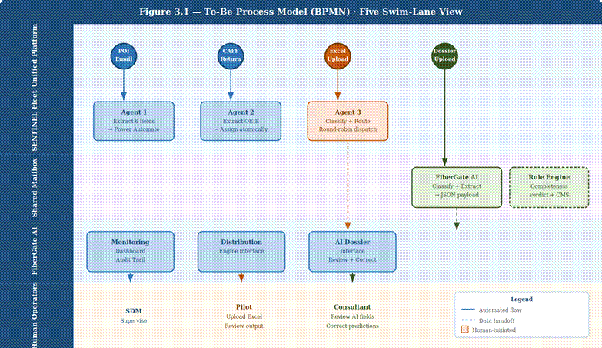
\includegraphics[width=0.52\textwidth,max width=\textwidth]{images/image18.png}
  \caption{BPMN to-be process model of the three automated workflows and their residual human touchpoints.}
  \label{fig:image18}
\end{figure}

\subsection{Operational Transformation Strategy}

The transformation strategy rests on the principle of graded automation: full autonomy for tasks whose inputs and decision rules are deterministic, confidence-gated assistance for tasks requiring semantic judgment, and preserved human control for tasks with strategic or relational consequences. Under this framework, Agents 1 and 2 operate without any human intervention on clearly structured email payloads. Agent 3 produces a human-reviewable distribution workbook before dispatching Planner tasks, ensuring the Pilot retains authority over assignment decisions. The AI Service routes uncertain field extractions to the consultant review queue rather than silently accepting them, preserving audit integrity.

The transformation also addresses the tool fragmentation problem directly. Rather than replacing individual tools, FiberGate wraps them: Power Automate continues to own SharePoint and Planner operations, Exchange remains the communication backbone, and the Unified Platform provides a single pane of glass over all operations without requiring migration of any existing data.

\section{Global Ecosystem Architecture}

\subsection{Three-Pillar Architectural Vision and Layered Design}

The FiberGate Ecosystem is structured as three vertically integrated pillars arranged in a layered dependency hierarchy. The Automation Layer (SENTINEL Fleet) executes deterministic, rule-based workflows against live operational data. The Intelligence Layer (FiberGate AI Service) provides probabilistic document understanding for dossiers that require semantic interpretation. The Governance Layer (Unified Platform) provides a unified operational surface for all human actors and exposes the control plane for both subordinate layers. Each layer communicates with adjacent layers only through authenticated REST contracts, ensuring that failure in one layer cannot cascade uncontrolled into others.

\begin{figure}[H]
  \centering
  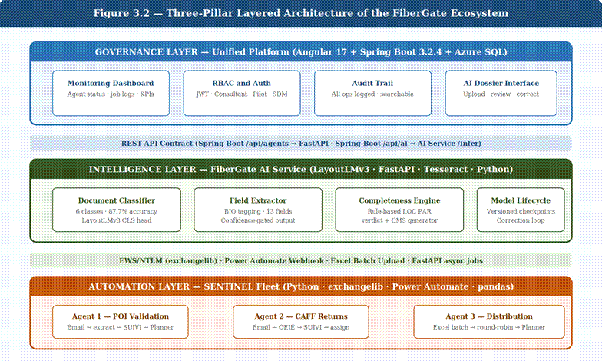
\includegraphics[width=0.52\textwidth,max width=\textwidth]{images/image19.png}
  \caption{FiberGate Ecosystem three-pillar architecture: Automation, Intelligence, and Governance layers.}
  \label{fig:image19}
\end{figure}

\subsection{Hybrid Event-Driven and Batch-Driven Processing Paradigm}

The ecosystem deliberately employs a hybrid processing model, because the operational cadence of each process differs materially. Agents 1 and 2 are event-driven: they run a 60-second Exchange polling loop and react immediately to new emails, achieving the sub-90-second latency target required to eliminate the same-day processing gap. Agent 3 is batch-driven on demand: it is triggered once per operational day by the Pilot after uploading the latest PAR France workbooks. The AI Service is synchronous request-response: it processes dossiers as they are uploaded by consultants throughout the working day. This model avoids the complexity of a unified messaging bus while satisfying the distinct timing requirements of each workflow.

\begin{table}[H]
  \centering
  \caption{Processing paradigm and human touchpoints by ecosystem component}
  \renewcommand{\arraystretch}{1.0}
  \footnotesize
  \begin{tabularx}{\textwidth}{|X|X|X|X|}
    \hline
    \textbf{Component} & \textbf{Paradigm} & \textbf{Trigger} & \textbf{Human Touchpoint} \\ \hline
    Agent 1 POI Validation & Event-driven & New email in FINOI folder & None fully autonomous \\ \hline
    Agent 2 CAFF Returns & Event-driven & New email in \_retour CAFF & None fully autonomous \\ \hline
    Agent 3 Distribution & Batch on-demand & Pilot uploads Excel workbooks & Pilot reviews workbook before confirming dispatch \\ \hline
    FiberGate AI Service & Request-response & Consultant uploads dossier & Consultant reviews and corrects AI extractions \\ \hline
    Unified Platform & Reactive & User action or agent event & SDM: monitoring, audit review, user management \\ \hline
  \end{tabularx}
\end{table}

\subsection{Inter-Component Communication, Integration, and Data Flow}

All inter-component communication is conducted over authenticated HTTPS. No component holds a direct database connection other than the Spring Boot backend via its JPA private endpoint to Azure SQL. The Unified Platform is the sole caller of the FastAPI agent server and the AI Service; agents themselves call Power Automate webhooks directly without routing through the platform. This topology keeps the platform's responsibility limited to orchestration and audit, and prevents circular dependency between the automation and governance layers.

\begin{figure}[H]
  \centering
  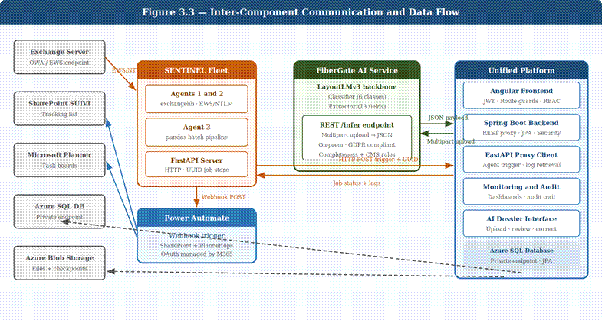
\includegraphics[width=0.52\textwidth,max width=\textwidth]{images/image20.png}
  \caption{Data flow diagram of authenticated communication paths across the FiberGate ecosystem.}
  \label{fig:image20}
\end{figure}

\section{Azure Cloud Architecture}

\subsection{Cloud Hosting Strategy and Resource Architecture}

All FiberGate components are hosted within a single Azure Virtual Network inside the Mantu Group subscription. The application tier hosts three compute resources: an App Service running the Spring Boot backend, an App Service running the FastAPI agent server, and an Azure Static Web App serving the Angular SPA via CDN. The AI inference VM is placed in the application subnet but assigned a private IP exclusively, making it unreachable from the public internet. The data tier is confined to a separate subnet and accessed exclusively through private endpoints, ensuring that the database and Blob Storage have zero public internet exposure. The design presented here reflects the target architecture defined during the Design phase; during implementation the compute and data tiers were consolidated onto Azure Container Apps and a managed PostgreSQL instance for the reasons set out at the start of Section~6.4.

\begin{figure}[H]
  \centering
  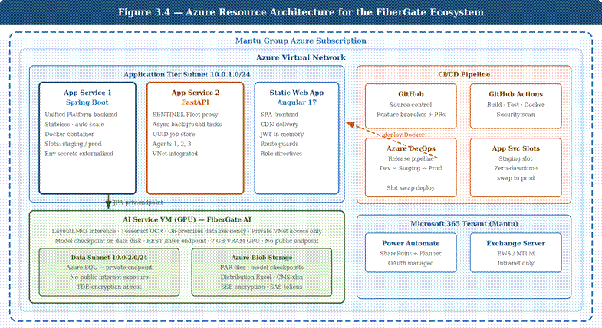
\includegraphics[width=0.52\textwidth,max width=\textwidth]{images/image21.png}
  \caption{Azure hosting architecture: App Services, AI inference VM, storage, CI/CD pipeline, and M365 tenant boundaries.}
  \label{fig:image21}
\end{figure}

\subsection{Service Topology, Network Security, and Scalability Design}

The NSG on the VNet boundary enforces an ingress-allow rule on port 443 only, denying all other inbound traffic. The AI Service VM and the data tier resources have no NSG rules permitting inbound traffic from outside the VNet. The Spring Boot App Service is configured with auto-scale rules that add instances when CPU utilisation exceeds 70\% for five consecutive minutes, supporting the anticipated increase in dossier submission volume following go-live. The FastAPI App Service is deliberately not auto-scaled, as concurrent agent executions share the same Exchange session context and must be serialised.

\begin{figure}[H]
  \centering
  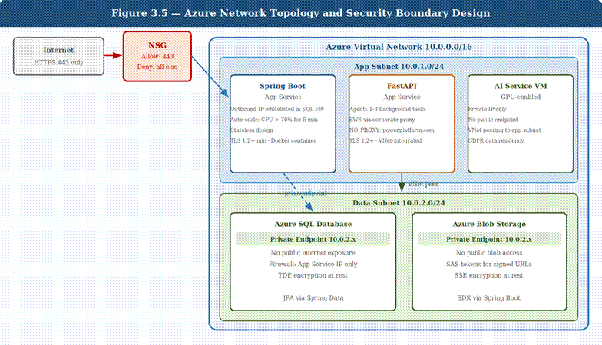
\includegraphics[width=0.52\textwidth,max width=\textwidth]{images/image22.png}
  \caption{Azure VNet topology with subnet segmentation, NSG boundary rules, private endpoints, and auto-scaling.}
  \label{fig:image22}
\end{figure}

\section{SENTINEL Fleet Conceptual Design}

\subsection{Architectural Design Principles: Zero-Oversight and Hybrid Automation}

The SENTINEL Fleet is governed by two design principles. The first is zero-oversight operation: once triggered, each agent must complete its full processing cycle without requiring human confirmation or intervention under normal conditions. The second is hybrid automation: agents use Python exchangelib for Exchange interaction where no Power Platform connector was available and delegate SharePoint and Planner operations to Power Automate flows, which hold the required M365 OAuth credentials independently of the agent runtime. This hybrid model avoids the EWS proxy constraints that prevented direct SharePoint Graph API calls from the agent environment, while maintaining a clean audit trail for all M365 operations executed by Power Automate on behalf of the agent.

\subsection{Shared Infrastructure Design and Email Listener Architecture}

All three agents instantiate a common five-stage execution skeleton: Exchange connection with NTLM authentication and proxy configuration, mailbox navigation and unread email enumeration, payload extraction and validation, Power Automate webhook dispatch with error handling, and mark-as-read with state persistence. This skeleton is parameterised per agent through a configuration object rather than duplicated, enabling each agent to be restarted, monitored, and versioned independently. The FastAPI server exposes each agent as an asynchronous background task, returning a job UUID immediately on trigger and allowing the Unified Platform to poll for completion and retrieve structured logs.

\subsection{Per-Agent Conceptual Design: Agents 1, 2, and 3}

Agent 1 targets the FINOI Exchange folder and applies a multi-pattern regex engine to extract six mandatory fields from POI notification email bodies: AS code, OEIE identifier, Affaire reference, Etablissement name, PC code (alphanumeric pattern [0-9A-Z]+), and type\_demande. Rows containing the word anticipation in type\_demande are explicitly skipped, as they represent pre-notifications not yet subject to validation. Missing mandatory fields trigger a logged skip rather than an exception, preserving processing continuity for the remaining emails in the batch.

Agent 2 targets the \_retour CAFF folder and applies a single strict pattern to the email subject line to extract the OEIE identifier. The Power Automate flow triggered by Agent 2 is designed to be atomic: the SUIVI lookup, assignment update, and Planner task creation execute within a single flow invocation, eliminating the intermediate state in which a CAFF return has been seen but not yet assigned that caused the historical one-day processing delay.

Agent 3 operates as a batch distribution engine. It ingests the Full PAR France workbook, two Planner export files, and the previous distribution run's output. The six-step pandas pipeline classifies each dossier row by type\_demande (RAR, Nouvelle, Retour, GoLP, or Default), applies a continuity-of-treatment rule to preserve existing consultant assignments for in-progress dossiers, and distributes remaining rows using a round-robin algorithm with a persistent last\_assigned index that carries across daily runs. The output is a three-sheet workbook presented to the Pilot for review before dispatch. Agent 3 then sends one Power Automate webhook per row with a two-second inter-call delay, respecting the flow call rate limits of the M365 tenant.

\section{FiberGate AI Service Conceptual Design}

\subsection{Multimodal Document Processing Pipeline Overview}

The FiberGate AI Service implements a five-stage pipeline that transforms a raw PDF or image upload into a structured JSON payload containing document classifications, extracted field values with per-token confidence scores, a LOC PAR completeness verdict, and a pre-filled 27-column CMS Excel file. The first three stages are neural and depend on the LayoutLMv3 backbone. The final two stages are deterministic rule engines whose logic is independently maintainable: changes to LOC PAR requirements or CMS column mappings require no model retraining, only updates to the rule configuration.

\begin{figure}[H]
  \centering
  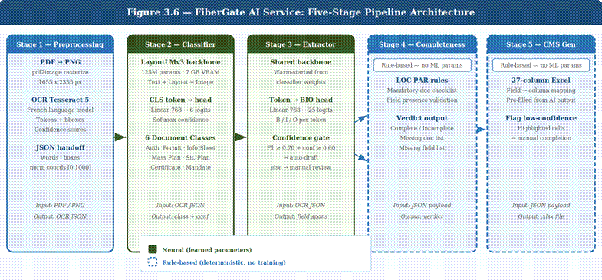
\includegraphics[width=0.52\textwidth,max width=\textwidth]{images/image23.png}
  \caption{Five-stage inference pipeline from document upload to CMS Excel output, gated by a confidence threshold.}
  \label{fig:image23}
\end{figure}

\subsection{Dataset Strategy and Field Extraction Workflow}

The training corpus was assembled from historical PAR dossiers collected over nine months of operational activity, covering the six document categories present in the LOC PAR workflow: authorisation permit, information sheet, mass plan, situation plan, technical certificate, and mandate. Documents were annotated at the token level using BIO tagging across twelve field types (a twenty-five-label BIO space) defined in consultation with the SDM and senior OSA consultants. Dataset imbalance across document classes was addressed through class-weighted loss during fine-tuning.

The confidence gate was empirically calibrated on the validation partition. Fields whose extraction head produces a per-token confidence below 0.60 or whose span-level F1 falls below 0.70 are written to the CMS output with a visual flag indicating mandatory consultant review. This gate ensures that the AI Service fails explicitly and visibly rather than silently, preserving the trust relationship between the system and its users that is essential for adoption in a regulated operational context.

\section{Unified Platform Conceptual Design}

\subsection{Platform Vision, Actor Identification, and Functional Modules}

The Unified Platform replaces the fragmented nine-tool interface with a single authenticated web application. Three actor roles are defined in a strict hierarchy: the Consultant handles dossier processing and AI review; the Pilot manages distribution operations and monitors agent executions; the SDM governs platform administration, user management, audit oversight, and AI model lifecycle. Each role inherits all capabilities of the role below it. The role hierarchy is enforced at two independent layers to prevent privilege escalation.

\begin{table}[H]
  \centering
  \caption{Unified Platform functional modules by primary actor}
  \renewcommand{\arraystretch}{1.0}
  \begin{tabularx}{\textwidth}{|X|X|X|}
    \hline
    \textbf{Module} & \textbf{Primary Actor} & \textbf{Key Capabilities} \\ \hline
    Authentication & All Roles & Login, JWT session management, forced password change on first login \\ \hline
    AI Dossier Interface & Consultant & Upload PAR dossier, view AI document classifications, review extracted field values, correct low-confidence predictions, download CMS Excel \\ \hline
    Distribution Management & Pilot & Upload Full PAR France and Planner export files, trigger Agent 3, download three-sheet distribution workbook, view workload statistics \\ \hline
    Agent Monitoring & Pilot / SDM & View all agent execution history, poll live job status, stream structured logs, review execution timeline \\ \hline
    User and Role Management & SDM & Create and deactivate user accounts, assign and modify role bindings, reset passwords \\ \hline
    Audit Trail & SDM & Search immutable audit log by actor, action type, entity, and date range; export filtered results to CSV \\ \hline
    KPI Dashboard & SDM & Configure date ranges, view throughput, processing time, and AI accuracy KPIs, compare pre- and post-FiberGate metrics \\ \hline
    AI Model Lifecycle & SDM & View model version history, review per-version accuracy and confidence reports, approve retraining cycle initiation \\ \hline
  \end{tabularx}
\end{table}

\subsection{Functional Architecture and Role-Based Access Control Model}

RBAC is enforced at two independent layers. In the Angular frontend, route guards prevent unauthorised navigation to protected views, and structural directives conditionally render UI elements based on the authenticated user's role claim. In the Spring Boot backend, Spring Security @PreAuthorize annotations on each REST endpoint validate the JWT role claim server-side before any service logic executes. The stateless JWT model means no server-side session table is required, simplifying horizontal scaling and reducing the attack surface.

\subsection{Integration Architecture and External Dependencies}

The Spring Boot backend acts as the single integration hub for all external systems accessible to the platform. It proxies agent triggers and log retrieval to the FastAPI server, forwards dossier uploads to the AI Service via a multipart REST call, and persists all result data to Azure SQL via Spring Data JPA through the private endpoint. The platform does not call Power Automate directly; that responsibility belongs exclusively to the SENTINEL agents. This separation ensures that the platform's audit trail reflects what the agents actually did, not what the platform instructed them to do.

\begin{figure}[H]
  \centering
  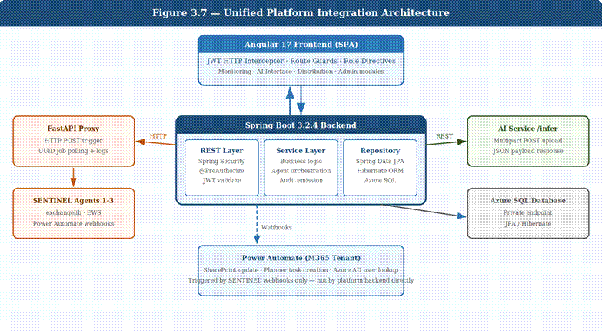
\includegraphics[width=0.52\textwidth,max width=\textwidth]{images/image24.png}
  \caption{Platform integration architecture and API contract boundaries across the FiberGate ecosystem.}
  \label{fig:image24}
\end{figure}

\section{UML System Specification}

The following UML diagrams constitute the formal system specification for the FiberGate Ecosystem. Each diagram is derived from the architectural and requirements decisions documented in sections 3.1 through 3.7, and represents the design contract for the implementation chapters that follow. Diagrams are presented in the order in which they would be consulted during implementation: global scope first, then per-component detail.

\subsection{Global Use Case Diagram}

The global use case diagram captures all actor-system interactions across the three pillars, partitioned by RBAC boundary zone. Autonomous agent processes triggered by the Exchange Server are shown as dashed-boundary use cases to distinguish them from platform-mediated interactions.

\begin{figure}[H]
  \centering
  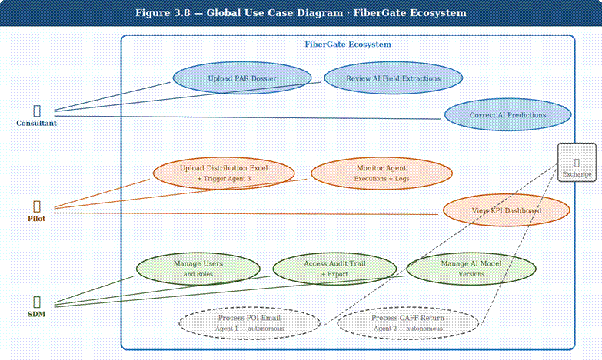
\includegraphics[width=0.52\textwidth,max width=\textwidth]{images/image25.png}
  \caption{Global use case diagram of the three actor roles and the autonomous SENTINEL agent processes.}
  \label{fig:image25}
\end{figure}

\subsection{Email Listener Orchestration Sequence Diagram}

The email listener sequence models the shared orchestration pattern common to Agents 1 and 2: asynchronous job spawning via FastAPI, the 60-second Exchange polling loop, regex extraction, Power Automate webhook dispatch, and mark-as-read state management. The platform polls the job endpoint for completion rather than blocking on the trigger call.

\begin{figure}[H]
  \centering
  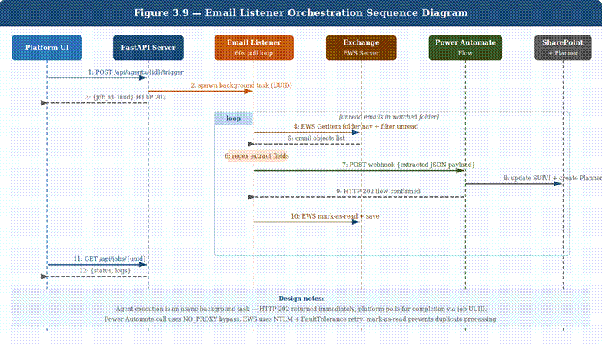
\includegraphics[width=0.52\textwidth,max width=\textwidth]{images/image26.png}
  \caption{Sequence diagram of the shared email listener and event-driven agent orchestration pattern.}
  \label{fig:image26}
\end{figure}

\subsection{Agent 1, 2, and 3 Sequence Diagrams}

The three agent sequence diagrams specify per-agent workflows in detail, including error branches, conditional logic, and atomicity guarantees specific to each agent.

\begin{figure}[H]
  \centering
  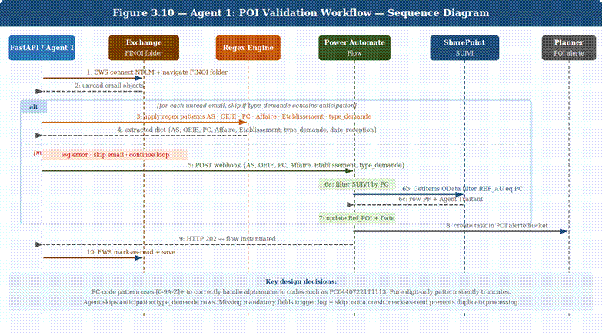
\includegraphics[width=0.52\textwidth,max width=\textwidth]{images/image27.png}
  \caption{Agent 1 sequence: FINOI folder polling, regex field extraction, and Planner task creation.}
  \label{fig:image27}
\end{figure}

\begin{figure}[H]
  \centering
  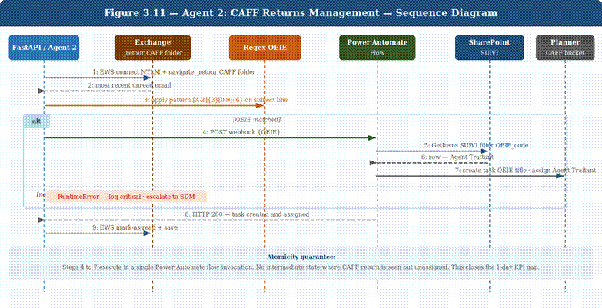
\includegraphics[width=0.52\textwidth,max width=\textwidth]{images/image28.png}
  \caption{Agent 2 sequence: CAFF folder polling, OEIE pattern matching, and atomic flow execution.}
  \label{fig:image28}
\end{figure}

\begin{figure}[H]
  \centering
  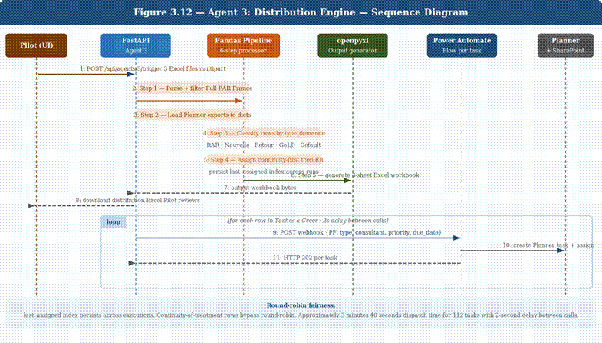
\includegraphics[width=0.52\textwidth,max width=\textwidth]{images/image29.png}
  \caption{Agent 3 sequence: pandas processing pipeline, workbook generation, and webhook dispatch loop.}
  \label{fig:image29}
\end{figure}

\subsection{FiberGate AI Service Sequence Diagram}

The AI Service sequence diagram models the full inference pipeline from dossier upload to CMS download, annotating the boundary between the neural backbone stages and the deterministic rule engine stages. The on-premises data residency guarantee is explicitly annotated: no document data crosses this boundary.

\begin{figure}[H]
  \centering
  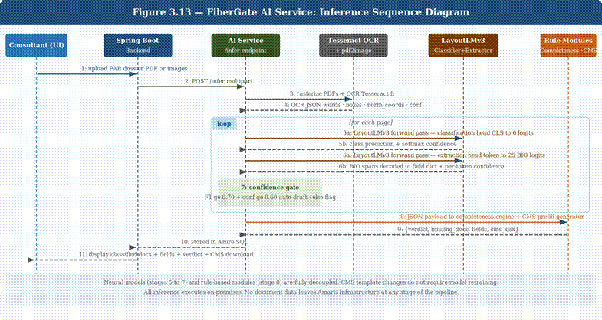
\includegraphics[width=0.52\textwidth,max width=\textwidth]{images/image30.png}
  \caption{Sequence diagram for the AI Service five-stage inference pipeline.}
  \label{fig:image30}
\end{figure}

3.8.5 Unified Platform Use Case and Sequence Diagrams

The Unified Platform use case diagram annotates each use case with its RBAC access zone. The four representative interaction scenarios in Figure 3.15 cover the primary workflows of each actor role and illustrate the asynchronous job polling model, the audit trail query flow, and the AI review correction cycle. The lower panel of Figure 3.15 provides a consolidated functional module summary by role for reference during implementation.

\begin{figure}[H]
  \centering
  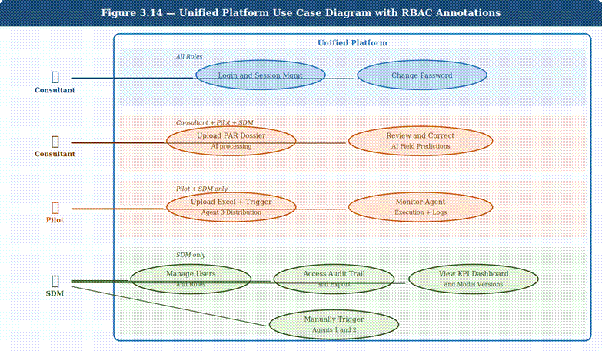
\includegraphics[width=0.52\textwidth,max width=\textwidth]{images/image31.png}
  \caption{Unified Platform use case diagram partitioned into four colour-coded RBAC zones.}
  \label{fig:image31}
\end{figure}

\begin{figure}[H]
  \centering
  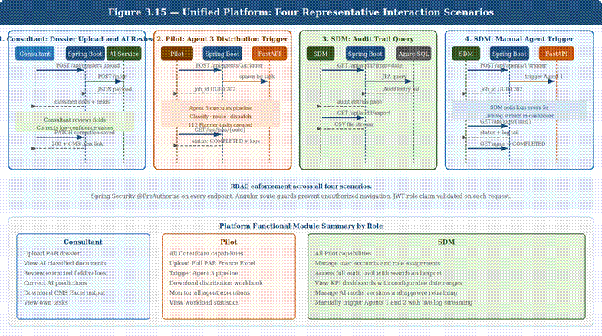
\includegraphics[width=0.52\textwidth,max width=\textwidth]{images/image32.png}
  \caption{Sequence diagrams for four representative role-based platform scenarios.}
  \label{fig:image32}
\end{figure}

\subsection{Unified Platform Class and Component Diagrams}

The domain class diagram specifies all persistent entities, their attributes, and their relationships. The component diagram specifies the architectural boundaries, provided and required interfaces, and the seven design principles governing inter-component communication that must be preserved throughout implementation.

\begin{figure}[H]
  \centering
  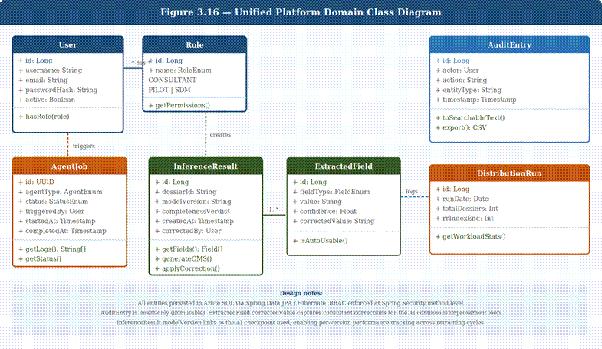
\includegraphics[width=0.52\textwidth,max width=\textwidth]{images/image33.png}
  \caption{Domain class diagram of the platform's core entities and their relationships.}
  \label{fig:image33}
\end{figure}

\begin{figure}[H]
  \centering
  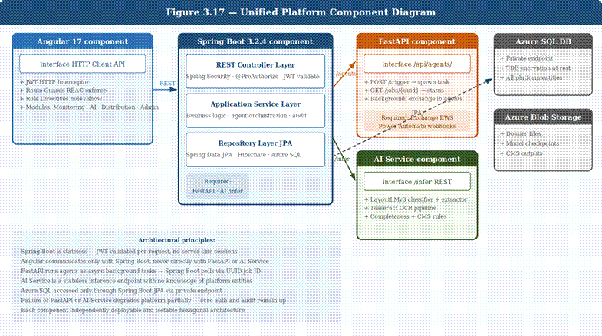
\includegraphics[width=0.52\textwidth,max width=\textwidth]{images/image34.png}
  \caption{Component diagram of the platform's tiers, interfaces, and underlying architectural principles.}
  \label{fig:image34}
\end{figure}

\subsection{Ecosystem Deployment Diagram}

The ecosystem deployment diagram maps all runtime artefacts to their physical or virtual execution environments within the Azure VNet. Network paths, CI/CD deployment flows, and M365 tenant integration boundaries are annotated to provide a complete picture of the production topology.

\begin{figure}[H]
  \centering
  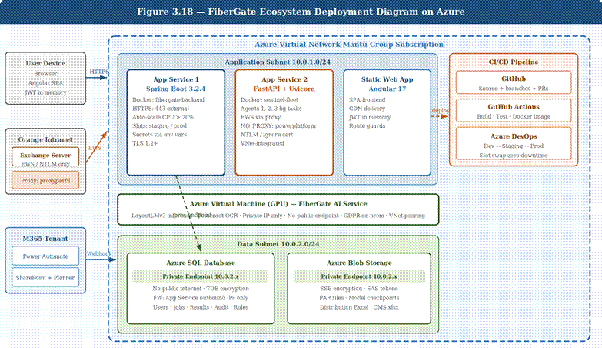
\includegraphics[width=0.52\textwidth,max width=\textwidth]{images/image35.png}
  \caption{Deployment diagram of FiberGate artefacts within the Azure VNet and CI/CD pipeline.}
  \label{fig:image35}
\end{figure}

\section*{Conclusion}
\addcontentsline{toc}{section}{Conclusion}

This chapter has presented the complete system analysis and conceptual design for the FiberGate Ecosystem. The requirements engineering phase produced a formalised baseline of eleven functional requirements, ten non-functional requirements, six hard technical constraints, and a five-risk design register, all traceable to the operational problem statement established in Chapter 2.

The target process model confirmed that the five identified bottlenecks can be systematically addressed: full autonomy for event-driven POI and CAFF processing, batch automation with human review for distribution, and confidence-gated AI assistance for dossier completeness verification. The hybrid event-driven and batch-driven processing paradigm was selected precisely because the operational cadence of each process differs in a way that makes a unified messaging model unnecessarily complex and fragile.

The three-pillar architecture separates automation, intelligence, and governance into independently deployable and independently maintainable components, communicating only through authenticated REST contracts. The Azure cloud architecture places all data behind private endpoints, restricts inbound traffic to HTTPS 443 at the NSG boundary, and ensures that no PAR dossier data leaves the Amaris infrastructure at any stage of processing. The CI/CD pipeline provides zero-downtime deployment through App Service slot swapping, reducing deployment risk in a production environment with strict availability requirements.

The UML specification comprising eighteen diagrams provides the design contract for the implementation work detailed in the chapters that follow. Chapter 4 covers the design and implementation of the SENTINEL Automation Fleet. Chapter 5 addresses the FiberGate AI Service, from dataset construction through model architecture, training methodology, and experimental evaluation. Chapter 6 presents the Unified Platform implementation, Azure deployment, and the business impact assessment that validates the ecosystem against the KPIs established in the problem statement.
